\documentclass[a4paper,12pt,UTF8]{article}
\usepackage{CTEX}
\usepackage{graphicx}
\usepackage{diagbox}
\usepackage{tikz}
\usepackage{setspace}
\usepackage{subfigure}
\usepackage{indentfirst}
\usepackage{listings}
\usepackage{xcolor}

\lstset{
    basicstyle=\tt,
    %行号
    numbers=left,
    rulesepcolor=\color{red!20!green!20!blue!20},
    %escapeinside=``,
    %xleftmargin=0em,xrightmargin=5em, aboveskip=5em,
    %背景框
    framexleftmargin=1.5mm,
    frame=shadowbox,
    %背景色
    backgroundcolor=\color[RGB]{245,245,244},
    %样式
    keywordstyle=\color{blue}\bfseries,
    identifierstyle=\bf,
    numberstyle=\color[RGB]{0,192,192},
    commentstyle=\it\color[RGB]{96,96,96},
    stringstyle=\rmfamily\slshape\color[RGB]{128,0,0},
    %显示空格
    showstringspaces=false
}
\begin{document}
    \begin{spacing}{2.0}
        \title{\textbf{\huge{人工智能课程设计实验报告}}}
        \date{}
        \maketitle
        \begin{figure}[h]
            \centering
        
\includegraphics[width=7cm,height=7cm]{tongji_logo}
        \end{figure}
    \end{spacing}   
    {
    \Large
        \textbf{
        \begin{flushleft}
        学\hspace{1cm}号:\hspace{4cm}2151769\\
        姓\hspace{1cm}名:\hspace{4cm}吕博文\\
        专\hspace{1cm}业:\hspace{3cm}计算机科学与技术\\
        授课老师:\hspace{4cm}王俊丽\\
        \end{flushleft}
        }
    }
\newpage
\begin{center}
\Large{
        \textbf{Project0\\}
    }
\end{center}
\begin{flushleft}
    {
       \large{
            \textbf{1、实验内容\\}
            
       }
       \normalsize{
        \hspace{1cm}本次实验主要内容为搭建实验环境和简单熟悉python语言,为接下来
        的项目做好准备,本学期的实验环境主要采用python 3.6的环境,我们采用conda
        搭建一个属于自己的虚拟实验环境,并在该实验环境中完成对代码的编写和运行。\\
       }
       \large{
        \textbf{2、实验项目代码\\}
       }
       \normalsize{
            \textbf{2.1 addition.py\\}
       }
       \scriptsize{
        \begin{lstlisting}
def add(a, b):
    "Return the sum of a and b"
    "*** YOUR CODE HERE ***"

    return a+b        
        \end{lstlisting}                   
       }

       \normalsize{
            \textbf{2.2 buyLotsOfFruit.py\\}
       }
       \scriptsize{
        \begin{lstlisting}
from __future__ import print_function

fruitPrices = {'apples': 2.00, 'oranges': 1.50, 'pears': 1.75,
                'limes': 0.75, 'strawberries': 1.00}


def buyLotsOfFruit(orderList):
    """
        orderList: List of (fruit, numPounds) tuples

    Returns cost of order
    """
    totalCost = 0.0
    "*** YOUR CODE HERE ***"
    for index in range(len(orderList)):
        if orderList[index][0] in fruitPrices:
            totalCost=totalCost+orderList[index][1]*fruitPrices[orderList[index][0]]
        else:
            print('The fruit %s is not in the fruit shop!'%(orderList[index]))
            return None
    return totalCost


# Main Method
if __name__ == '__main__':
    "This code runs when you invoke the script from the command line"
    orderList = [('apples', 2.0), ('pears', 3.0), ('limes', 4.0)]
    print('Cost of', orderList, 'is', buyLotsOfFruit(orderList))
        \end{lstlisting}                   
       }

       \normalsize{
        \textbf{2.3 shopSmart.py\\}
       
       }
       \scriptsize{
        \begin{lstlisting}
from __future__ import print_function
import shop

def shopSmart(orderList, fruitShops):
    """
        orderList: List of (fruit, numPound) tuples
        fruitShops: List of FruitShops
    """
    "*** YOUR CODE HERE ***"
    shop_index=0;
    for index in range(len(fruitShops)):
        if index == 0:
            shop_index=0
        elif fruitShops[index].getPriceOfOrder(orderList)<fruitShops[shop_index].getPriceOfOrder(orderList):
            shop_index=index
    return fruitShops[shop_index]


if __name__ == '__main__':
    "This code runs when you invoke the script from the command line"
    orders = [('apples', 1.0), ('oranges', 3.0)]
    dir1 = {'apples': 2.0, 'oranges': 1.0}
    shop1 = shop.FruitShop('shop1', dir1)
    dir2 = {'apples': 1.0, 'oranges': 5.0}
    shop2 = shop.FruitShop('shop2', dir2)
    shops = [shop1, shop2]
    print("For orders ", orders, ", the best shop is", shopSmart(orders, shops).getName())
    orders = [('apples', 3.0)]
    print("For orders: ", orders, ", the best shop is", shopSmart(orders, shops).getName())
        \end{lstlisting}
       }
       \large{
        \textbf{3、实验结果\\}
        \begin{figure}[h]
            \centering
        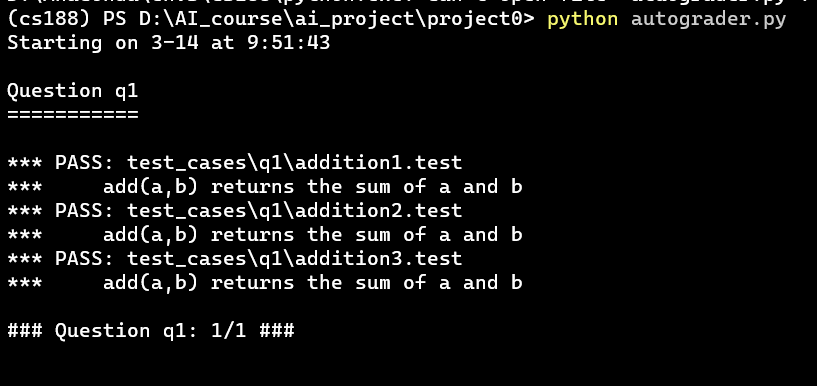
\includegraphics[width=12cm,height=7cm]{1}
        \end{figure}
        \begin{figure}[h]
            \centering
        
\includegraphics[width=12cm,height=7cm]{2}
        \end{figure}
        \begin{figure}[h]
            \centering
        
\includegraphics[width=12cm,height=7cm]{3}
        \end{figure}
        \begin{figure}[h]
            \centering
        
\includegraphics[width=12cm,height=7cm]{4}
        \end{figure}
       }
    }
\end{flushleft}
\end{document}

